%% Exercice 4

%\ExoSpecs{\TTBF{CalculTVA.sh}}{\TTBF{\RenduDir/src/exo1/}}{750}{640}{\TTBF{write}}
\ExoSpecsCustom{\TTBF{bt\_bst.c}}{\TTBF{\RenduDir/src/}}{750}{640}{Fonctions autorisées}{\TTBF{malloc(3)}, \TTBF{free(3)}, \TTBF{memcpy(3)}, \TTBF{printf(3)}}

\vspace*{0.7cm}

\noindent \ExoObjectif{Le but de l'exercice est d'implémenter une mini bibliothèque d'arbres binaires de recherche h-équilibrés sous forme d'arbres AVL.}

\bigskip

%\noindent Les fonctions demandées dans cet exercice devront se trouver dans une bibliothèque nommée \TTBF{libmystack}.
%Après un appel à la commande \texttt{make} à la racine du projet, il faut que votre chaîne de compilation produise à la racine de votre projet une version statique de la bibliothèque (qui se nommera \TTBF{libmystack.a}) ainsi qu'une version dynamique de la bibliothèque (qui se nommera \TTBF{libmystack.so}).
%
%\bigskip

\noindent Vous devez écrire plusieurs fonctions permettant d'effectuer des recherche, insertions, et suppressions de nœuds dans des ABR.
Un fichier \TTBF{bt\_avl.h} contenant toutes les fonctions exportables à implémenter vous est fourni en annexe.
Celui-ci implique de recoder une grande partie des fonctions précédentes, car un champs supplémentaire est requis pour simplifier la gestion de l'équilibrage.
Vous avez tout à fait le droit de recopier votre propre code des exercices précédents et le modifier légèrement pour prendre en charge l'équilibrage.
Typiquement, le type \TTBF{bt\_p} est modifié pour devenir \TTBF{avl\_p}.


\bigskip

%\noindent Conceptuellement, les fonctions manipulant des piles de type \TTBF{stack\_ll*} devront pouvoir gérer ces 3 cas :

%\bigskip

%\begin{center}
%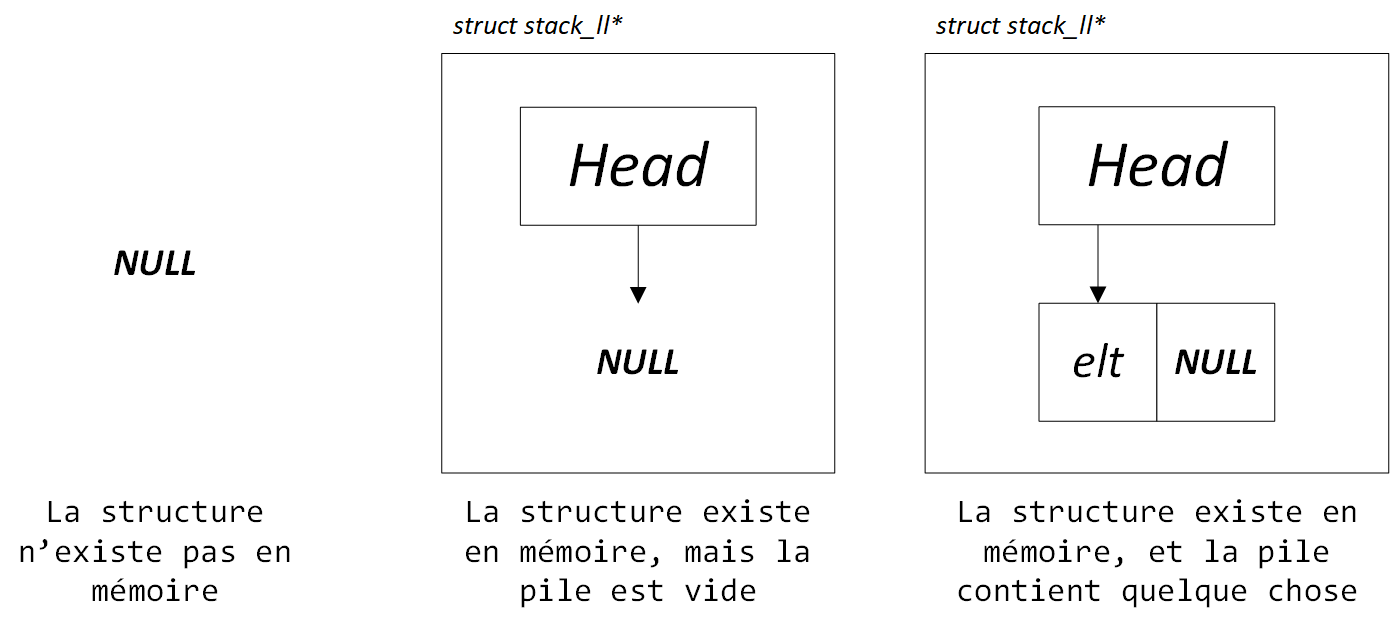
\includegraphics[scale=0.85]{Cours/Piles_Implementation_LL.png}
%\end{center}

\bigskip
%\newpage

\noindent Vous devez implémenter les fonctions suivantes :

\bigskip

\lstset{language=C}
%\begin{lstlisting}[frame=single,title={Liste des fonctions pour une pile avec liste chaînée}]
\begin{lstlisting}[frame=single]
avl_p *rot_r_bt_p(avl_p *node, avl_t *T);
avl_p *rot_l_bt_p(avl_p *node, avl_t *T);

avl_p *rot_rl_bt_p(avl_p *node, avl_t *T);
avl_p *rot_lr_bt_p(avl_p *node, avl_t *T);

avl_p *insert_avl_p(int key,
                    int len_elt,
                    void *elt,
                    avl_p *T);

avl_p *remove_avl_p(int key, avl_p *T);

int 
\end{lstlisting}


\subsubsection*{\TTBF{bt\_p *search\_bt\_p(int key, bt\_p *T)}}

\noindent Cette fonction recherche un nœud à partir de sa clé dans un arbre binaire.
Si la clé est trouvée, on renvoie un pointeur vers le nœud contenant la clé.
Si la clé n'est pas trouvée, ou que le l'arbre binaire est \TTBF{NULL}, alors la fonction doit renvoyer un pointeur \TTBF{NULL}.

\bigskip


\subsubsection*{\TTBF{bt\_p *insert\_leaf\_bt\_p(int key, int len\_elt, void *elt, bt\_p *T)}}

\noindent Cette fonction insère un nouvel élément et sa clé dans l'arbre binaire donné en paramètre.
L'insertion doit être faite en feuille.
Si l'arbre binaire en paramètre est vide, vous devez le créer et lui allouer un premier nœud qui servira de racine.

\bigskip


\subsubsection*{\TTBF{bt\_p *remove\_node\_bt\_p(int key, bt\_p *T)}}

\noindent Cette fonction supprime un nœud de l'arbre binaire donné en paramètre à partir de la clé également donnée en paramètre.
Vous devez libérer correctement la mémoire en libérant le nœud, mais sans libérer l'élément stocké dans le nœud (c'est à l'utilisateur de s'en charger).
Si l'arbre donné en paramètre est \TTBF{NULL}, la fonction doit renvoyer \TTBF{NULL}.

\bigskip


\subsubsection*{\textbf{[BONUS] }\TTBF{bt\_p *insert\_root\_cut\_bt\_p(int key, int len\_elt, void *elt, bt\_p *T)}}

\noindent Cette fonction insère un nouvel élément et sa clé dans l'arbre binaire donné en paramètre.
L'insertion doit être faite en racine avec la méthode de coupe.
Si l'arbre binaire en paramètre est vide, vous devez le créer et lui allouer un premier nœud qui servira de racine.
